\documentclass{article}
\usepackage[final]{nips_2017}
\usepackage[utf8]{inputenc} % allow utf-8 input
\usepackage[T1]{fontenc}    % use 8-bit T1 fonts
\usepackage[ngerman]{babel}
\usepackage{hyperref}       % hyperlinks
\usepackage{url}            % simple URL typesetting
\usepackage{booktabs}       % professional-quality tables
\usepackage{amsfonts}       % blackboard math symbols
\usepackage{nicefrac}       % compact symbols for 1/2, etc.
\usepackage{microtype}      % microtypography
\usepackage{graphicx}
\usepackage{placeins}       % \FloatBarrier
\title{Machine Learning for Computer Vision Abschlussprojekt: Rindenklassifizierung}

\author{
  Paul Walker\\
  Department of Computer Science\\
  DHBW Stuttgart\\
  \texttt{inf20045@dhbw-stuttgart.de} \\
  \And
  Tom Hofer\\
  Department of Computer Science\\
  DHBW Stuttgart\\
  \texttt{inf20173@lehre-dhbw-stuttgart.de} \\
}

\begin{document}

\begin{center}
\includegraphics[height=0.7cm]{DHBW_logo}
\end{center}

\maketitle

\begin{abstract}
  % The abstract should consist of 1 paragraph describing the motivation for your paper and a high-level explanation of the methodology you used/results obtained.
  Diese Arbeit befasst sich mit der Entwicklung eines Machine Learning Modells zur Klassifikation von Rinde zu bestimmten Baumarten. Das Modell könnte in der Praxis beispielsweise in einer App zur Bestimmung der Baumart anhand eines Fotos der Baumrinde eingesetzt werden. Im Rahmen der Arbeit werden vier Modelle basierend auf den vortrainierten Modellen InceptionV3, MobileNetV2, VGG16 und VGG19 erstellt, getestet und gegenübergestellt. Für das Training der Modelle kommen ein Trainingsset mit Daten aus dem Internet und ein Validationset mit selbst erhobenen Daten zum Einsatz.
\end{abstract}

\section{Einleitung}
%Explain the problem and why it is important. Discuss your motivation for pursuing this
%problem. Give some background if necessary. Clearly state what the input and output
%is. Be very explicit: “The input to our algorithm is an {image, amplitude, patient age,
%rainfall measurements, grayscale video, etc.}. We then use a {SVM, neural network, linear
%regression, etc.} to output a predicted {age, stock price, cancer type, music genre, etc.}.”
%This is very important since different teams have different inputs/outputs spanning different
%application domains. Being explicit about this makes it easier for readers. If you are using
%your project for multiple classes, add a paragraph explaining which components of the
%project were used for each class.
Unser Abschlussprojekt befasst sich mit der Entwicklung eines Machine Learning Modells zur Bestimmung der Baumart anhand eines Fotos der Baumrinde. Die Rinde eignet sich seht gut für die Bestimmung der Baumart, da diese, anders als zum Beispiel Blätter oder Früchte, unabhängig von der Jahreszeit ist. Die Eingabe für unseren Algorithmus ist also ein Bild. Zur Klassifizierung der Baumart verwenden wir ein vortrainiertes Convolutional Neural Network, welches wir für unseren Anwendungsfall anpassen. Die Ausgabe, beziehungsweise Vorhersage unseres Algorithmus ist die Art des Baumes, dessen Rinde auf dem Foto abgebildet ist.

\section{Stand der Technik}
%[Optional and seen as extension] You can find existing papers, and see how they are similar to and differ
%from your work. In your opinion, which approaches were clever/good? What is the stateof-the-art?
%Do most people perform the task by hand? This includes previous attempts by others at your problem,
%previous technical methods, or previous learning algorithms. Google Scholar is very useful
%for this: https://scholar.google.com/ (you can click “cite” and it generates MLA, APA,
%BibTeX, etc.)
\url{https://link.springer.com/chapter/10.1007/978-3-030-65414-6_15}

\section{Daten und Features}
%Describe your dataset: how many training/validation/test examples do you have? Is there
%any preprocessing you did? What about normalization or data augmentation? What is the
%resolution of your images? How is your time-series data discretized? Include a citation on
%where you obtained your dataset from. Depending on available space, show some examples
%from your dataset. You should also talk about the features you used. If you extracted
%features using Fourier transforms, word2vec, PCA,
%ICA, etc. make sure to talk about it. Try to include examples of your data in the report
%(e.g. include an image, show a waveform, etc.).

Unser Trainingsdatenset besteht aus 21491 Bildern von Rinde aus dem Internet. Diese beziehen wir von den Folgenden Quellen: \url{https://zenodo.org/record/4872489}, \url{https://zenodo.org/record/4446955} und \url{https://data.mendeley.com/datasets/zgr7r2r4nt/1}. Einige Beispile aus den Trainingsdaten sind in Abbildung~\ref{train} abgebildet. Für das Validationset haben wir 333 eigene Fotos aufgenommen. Einige Beispiele sind in Abbildung~\ref{validation} abgebildet. Ein Testset haben wir nicht, wir können also keine genaue Aussage über die tatsächliche Feldperformance unseres Modells treffen. Alle Bilder werden auf eine Grö\ss e von 512*512 Pixeln gebracht. Um Verzerrungen zu vermeiden werden die Grafiken zunächst durch Zuschneiden auf das richtige Seitenverhältnis gebracht. In unserem Validationset haben wir acht Klassen, beziehungsweise acht Baumarten. Wir nutzen von den Trainingsdaten nur die Arten, die auch im Validationset vorkommen. Zusätzlich wurden die Label der Trainingsdaten angepasst, da diese die Bäume noch in genaue unterarten einteilen, wir interessieren uns jedoch nur für die Überart. Die vertretenen Baumarten sind Esche, Buche, Birke, Tanne, Lärche, Eiche, Kiefer und Fichte.

\FloatBarrier

\begin{figure}[htbp!]
  \centering
  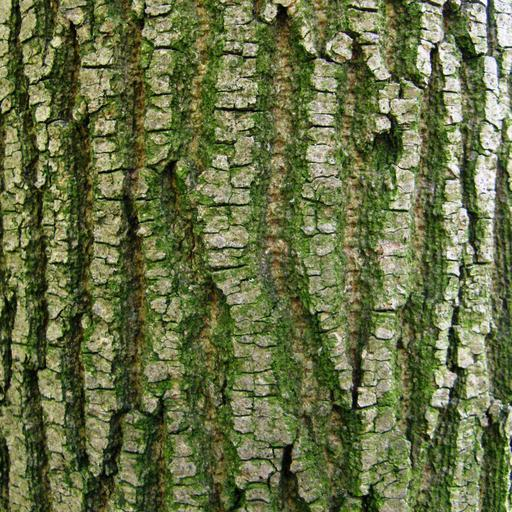
\includegraphics[width=0.24\linewidth]{examples/train/Ash}
  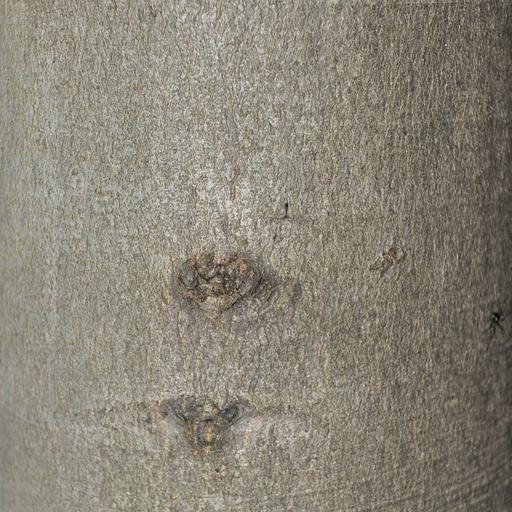
\includegraphics[width=0.24\linewidth]{examples/train/Beech}
  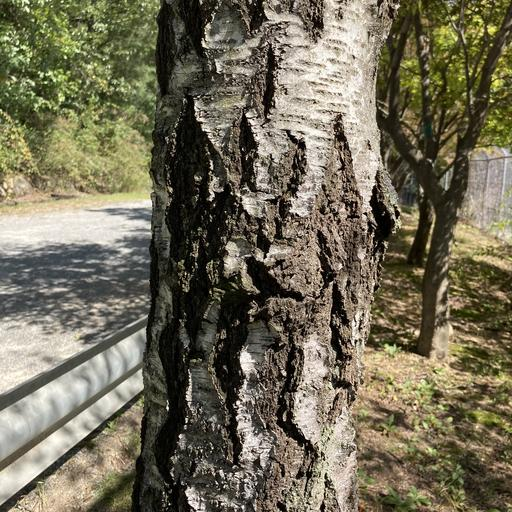
\includegraphics[width=0.24\linewidth]{examples/train/Birch}
  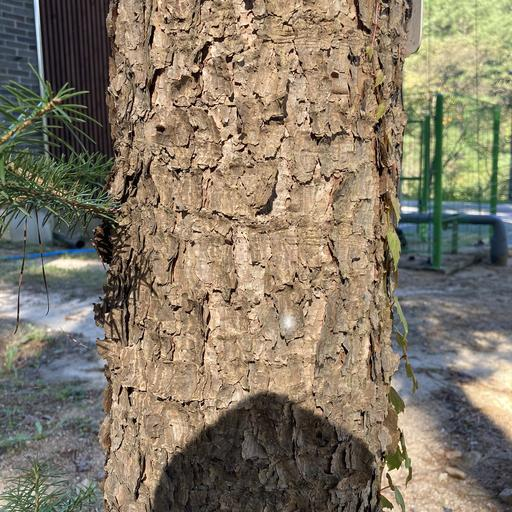
\includegraphics[width=0.24\linewidth]{examples/train/Fir}
  Esche \hspace{70pt} Buche \hspace{70pt} Birke \hspace{70pt} Tanne\\
  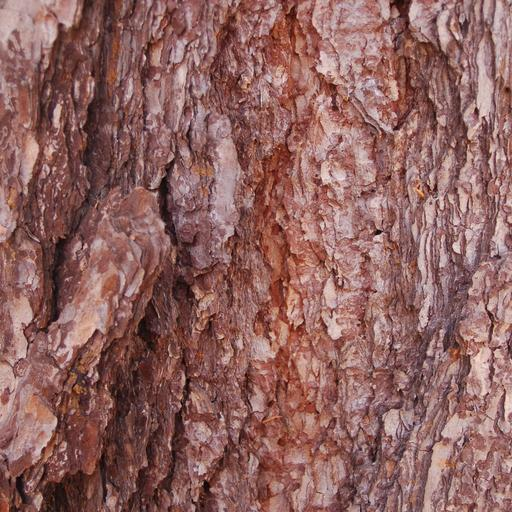
\includegraphics[width=0.24\linewidth]{examples/train/Larch}
  
\includegraphics[width=0.24\linewidth]{examples/train/Oak}
  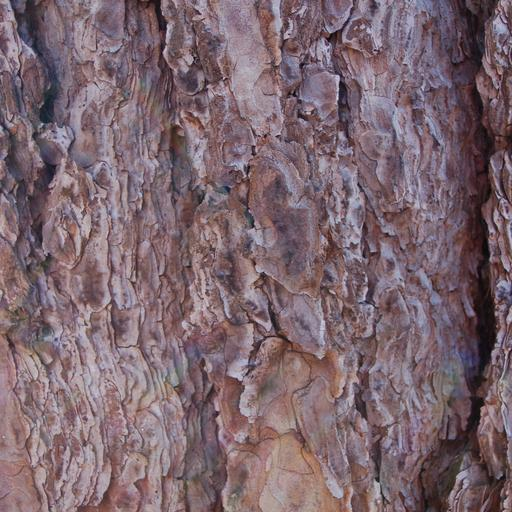
\includegraphics[width=0.24\linewidth]{examples/train/Pine}
  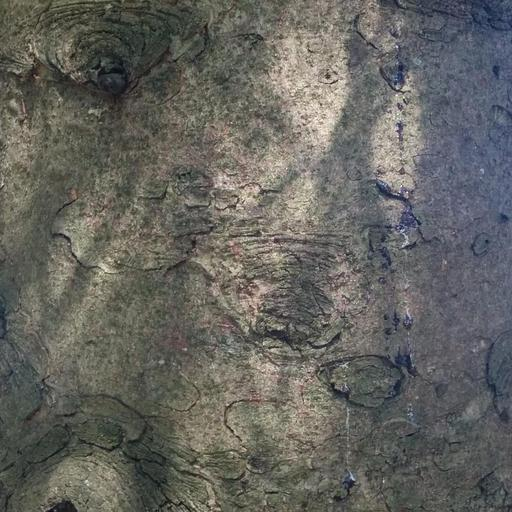
\includegraphics[width=0.24\linewidth]{examples/train/Spruce}
  Lärche \hspace{70pt} Eiche \hspace{70pt} Kiefer \hspace{70pt} Fichte\\
  \caption{Beispiele aus den Trainingsdaten}
  \label{train}
\end{figure}

\begin{figure}[htbp!]
  \centering
  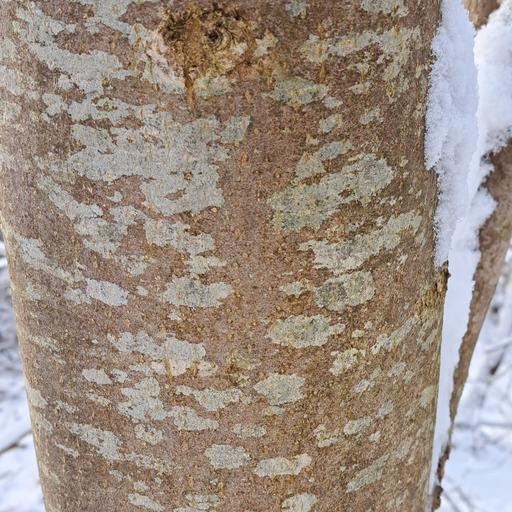
\includegraphics[width=0.24\linewidth]{examples/validation/Ash}
  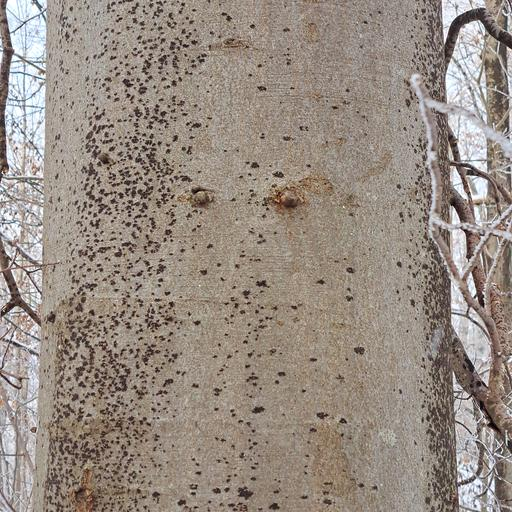
\includegraphics[width=0.24\linewidth]{examples/validation/Beech}
  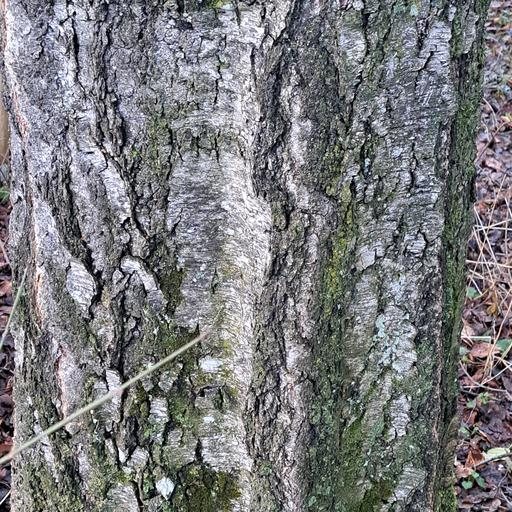
\includegraphics[width=0.24\linewidth]{examples/validation/Birch}
  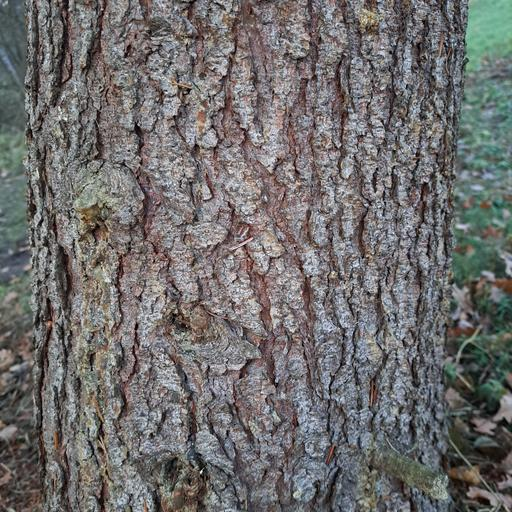
\includegraphics[width=0.24\linewidth]{examples/validation/Fir}
  Esche \hspace{70pt} Buche \hspace{70pt} Birke \hspace{70pt} Tanne\\
  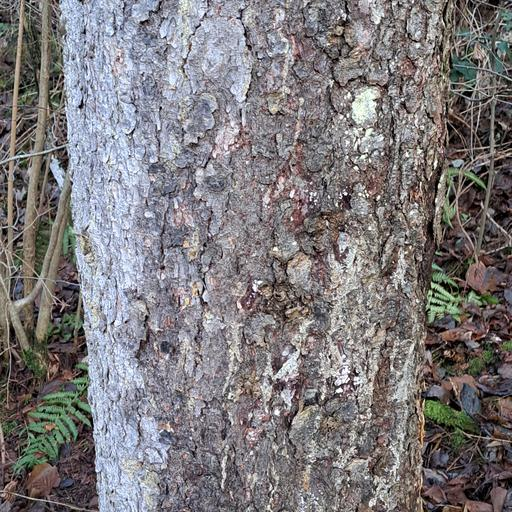
\includegraphics[width=0.24\linewidth]{examples/validation/Larch}
  
\includegraphics[width=0.24\linewidth]{examples/validation/Oak}
  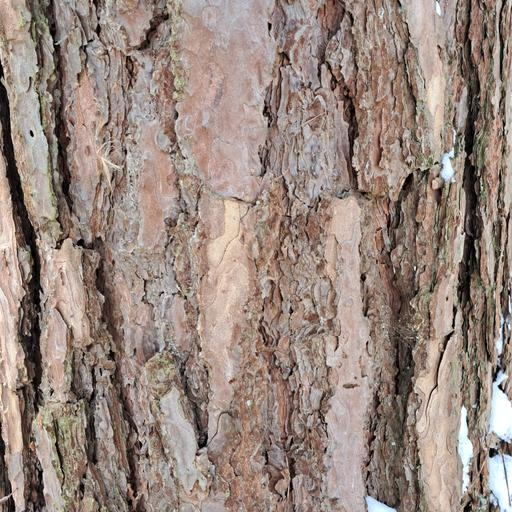
\includegraphics[width=0.24\linewidth]{examples/validation/Pine}
  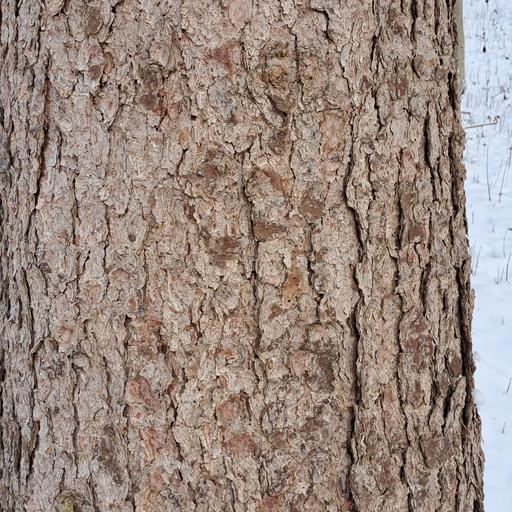
\includegraphics[width=0.24\linewidth]{examples/validation/Spruce}
  Lärche \hspace{70pt} Eiche \hspace{70pt} Kiefer \hspace{70pt} Fichte\\
  \caption{Baspiele aus dem Validationset}
  \label{validation}
\end{figure}

\section{Methoden}
%Describe your learning algorithms, proposed algorithm(s), or theoretical proof(s). Make
%sure to include relevant mathematical notation. For example, you can include the loss function you are using. It is okay to use formulas from the lectures (online or in-class). For each algorithm, give a short description 
%of how it works. Again, we are looking for your understanding of how these deep
%learning algorithms work. Although the teaching staff probably know the algorithms, future
%readers may not. Additionally, if you are
%using a niche or cutting-edge algorithm (anything else not covered in the class), you may want to explain your algorithm using 1/2
%paragraphs. Note: Theory/algorithms projects may have an appendix showing extended
%proofs (see Appendix section below).

Zur Erstellung unseres Modells verwenden wir Transfer learning. Das bedeutet wir verwenden ein bereits für Bilddaten Trainiertes Modell aus dem Internet und passen dieses auf unseren Anwendungsfall an. Die Anpassung erfolgt in den Ersten und letzten Schichten des Modells. Die erste Schicht wird auf unsere Eingabe, ein Bild mit 512*512 Pixeln und drei Kanälen, angepasst. Diese hinzugefügten Schichten sind beispielhaft in dem in Abbildung~\ref{VGG16} dargestelleten, auf VGG16 basierenden Modell, grün markiert. Au\ss erdem wird eine zweite Schicht eingefügt die ein Rescaling der Wertebereiche von 0 bis 255 auf einen Wertebereich von 0 bis 1 transformiert. Für die Ausgabe des Modells werden die letzten vier Shichten angepasst. Zunächst erfogt ein zeidimensionales global average pooling gefolgt von einer flatten und dense Schicht. Die dense Schicht verwendet eine Relu als Aktivierungsfunktion. In der letzten Schicht wird die Ausgabe des Modells nochmal auf die Anzahl an Klassen, also in unserem Fall acht, heruntergebrochen. Die Letzte Schicht ist ein Softmax-Layer. Diese Schichten sind in der Abbildung~\ref{VGG16} rot markiert.
\FloatBarrier
Wir verweden für unser Modell einen sparse categorial crossentropy loss.

\begin{figure}[htbp!]
  \centering
  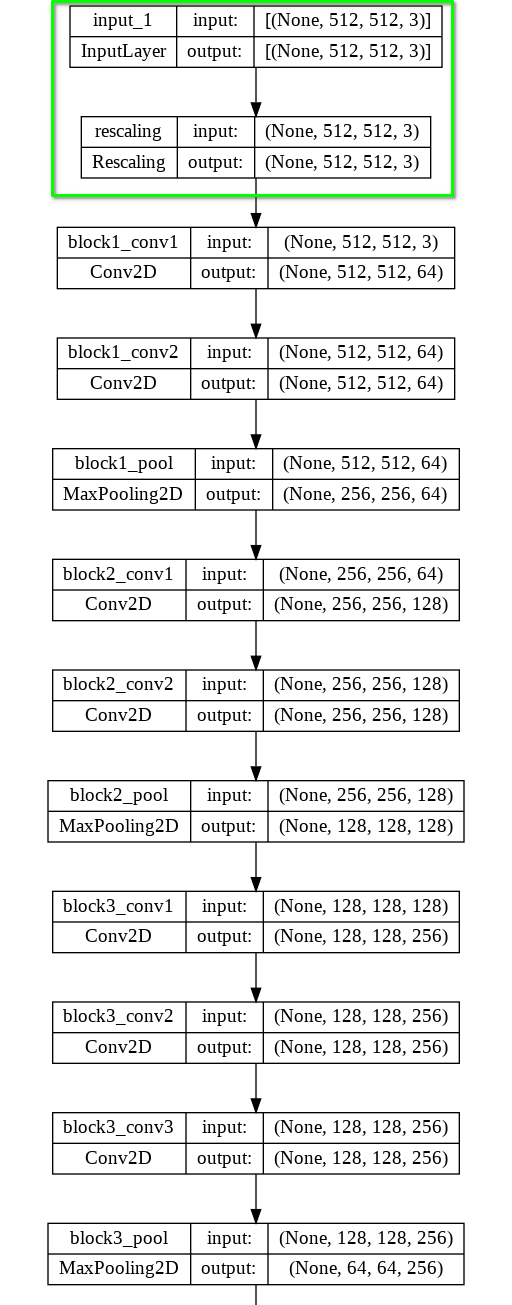
\includegraphics[width=0.4\linewidth]{VGG16_top}
  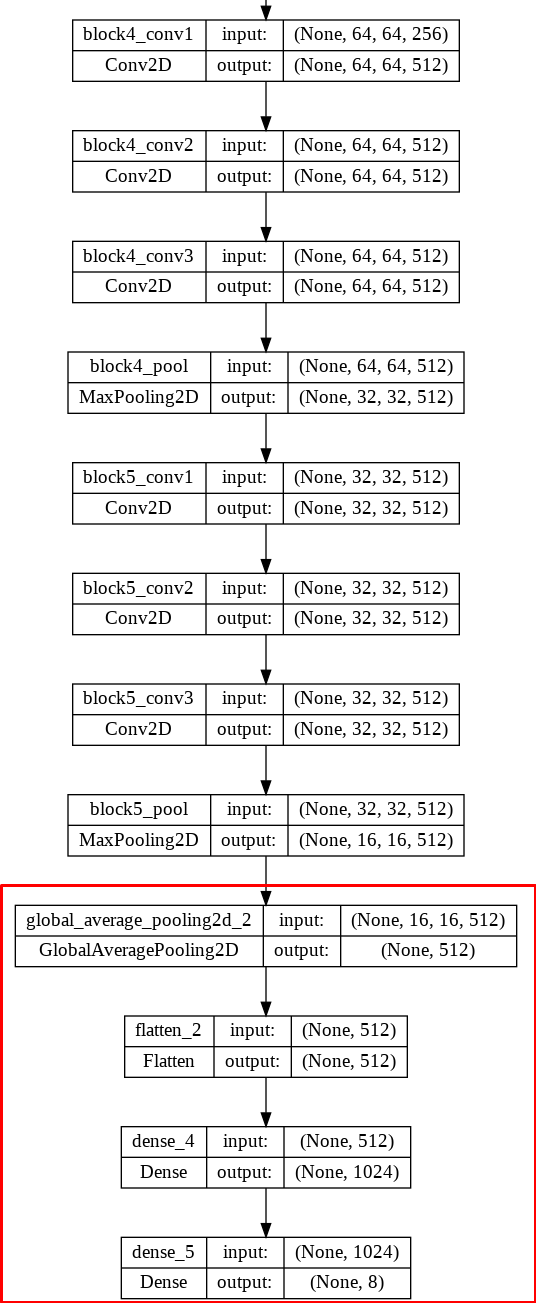
\includegraphics[width=0.4\linewidth]{VGG16_bottom}
  \caption{Darstellung des auf VGG16 basierenden Modells}
  \label{VGG16}
\end{figure}

\section{Experimente/Ergebnisse/Diskussion}
%You should also give details about what (hyper)parameters you chose (e.g. why did you
%use X learning rate for gradient descent, what was your mini-batch size and why) and how
%you chose them. What your primary metrics are: accuracy, precision,
%AUC, etc. Provide equations for the metrics if necessary. For results, you want to have a
%mixture of tables and plots. If you are solving a classification problem, can include a
%confusion matrix. Include performance metrics such as precision,
%recall, and accuracy. For regression problems, state the average error. You should have
%both quantitative and qualitative results. To reiterate, you must have both quantitative
%and qualitative results! If it applies: include visualizations of results, heatmaps,
%examples of where your algorithm failed and a discussion of why certain algorithms failed
%or succeeded. In addition, explain whether you think you have overfit to your training set
%and what, if anything, you did to mitigate that. Make sure to discuss the figures/tables in
%your main text throughout this section. Your plots should include legends, axis labels, and
%have font sizes that are legible when printed.

Wir haben verschiedene vortrainierte Basismodelle ausprobiert und deren Performance gegenübergestellt. Die betrachteten vortrainierten Modelle sind InceptionV3, MobileNetV2, VGG16 und VGG19.

\section{Fazit und Ausblick}
%Summarize your report and reiterate key points. Which algorithms were the highestperforming?
%Why do you think that some algorithms worked better than others? For
%future work, if you had more time, more team members, or more computational resources,
%what would you explore?


\section*{Referenzen}
%This section should include citations for: (1) Any papers mentioned in the related work
%section. (2) Papers describing algorithms that you used which were not covered in class.
%(3) Code or libraries you downloaded and used. This includes libraries such as scikit-learn, Tensorflow, Pytorch, Keras etc. Acceptable formats include: MLA, APA, IEEE. If you
%do not use one of these formats, each reference entry must include the following (preferably
%in this order): author(s), title, conference/journal, publisher, year. If you are using TeX,
%you can use any bibliography format which includes the items mentioned above. We are excluding
%the references section from the page limit to encourage students to perform a thorough
%literature review/related work section without being space-penalized if they include more
%references. Any choice of citation style is acceptable
%as long as you are consistent.
\subsection*{Libraries used}
\begin{itemize}
\item Pillow-SIMD
\item google.colab (drive)
\item Tensorflow
\item os
\item Keras
\item matplotlib
\end{itemize}

\medskip
\small
%[1] Alexander, J.A.\ \& Mozer, M.C.\ (1995) Template-based algorithms
%for connectionist rule extraction. In G.\ Tesauro, D.S.\ Touretzky and
%T.K.\ Leen (eds.), {\it Advances in Neural Information Processing
%  Systems 7}, pp.\ 609--616. Cambridge, MA: MIT Press.

%[2] Bower, J.M.\ \& Beeman, D.\ (1995) {\it The Book of GENESIS:
%  Exploring Realistic Neural Models with the GEneral NEural SImulation
%  System.}  New York: TELOS/Springer--Verlag.

%[3] Hasselmo, M.E., Schnell, E.\ \& Barkai, E.\ (1995) Dynamics of
%learning and recall at excitatory recurrent synapses and cholinergic
%modulation in rat hippocampal region CA3. {\it Journal of
%  Neuroscience} {\bf 15}(7):5249-5262.

\end{document}